% ─── Chapter 4: Results & Analysis ─────────────────────────────────
\chapter{Results \& Analysis}
\label{ch:results}

This chapter presents the experimental outcomes of the training pipeline.
Results are reported for two distinct settings: \textbf{fixed teams}
(Milestone~1) and \textbf{random teams} (Milestone~2).  We first define the
evaluation metric, then trace the development progression chronologically,
and finally assess each milestone independently.

\section{Benchmark Metric}

All validation results use the \textbf{benchmark protocol} (3~opponents
$\times$ 50~episodes $=$ 150~total).  The primary metric is the
\textbf{skill score}, a weighted average of per-opponent win rates:

\[
  \text{skill\_score} = \frac{
    1.0 \times \text{WR}_{\text{random}} +
    1.5 \times \text{WR}_{\text{random\_no\_switch}} +
    2.0 \times \text{WR}_{\text{heuristic}}
  }{1.0 + 1.5 + 2.0}
\]

Skill score ranges from 0 (loses all) to 1 (wins all).  The weighting
reflects opponent difficulty: beating the heuristic opponent contributes
twice as much as beating the random opponent.  Per-opponent win rates are
reported with Wilson 95\,\% confidence intervals.

\section{Development Progression}

This section traces the experimental outcomes chronologically, corresponding
to the development phases described in
Section~\ref{sec:dev_methodology}.  Note that the early phases used a
different curriculum configuration from the current four-stage system
(Section~\ref{sec:curriculum}): the early setup had two stages, ``easy''
(random opponents only) and ``medium'' (50/50 random and heuristic).

\subsection{Baseline Results}

With the initial system (22-action space, hash-based embeddings, 4-layer
post-norm transformer, no positional encoding), the training pipeline ran
end-to-end but produced limited learning:

\begin{itemize}
  \item \textbf{Easy stage} (random opponents only): promoted at
        ${\sim}$84K steps with 85\,\% win rate.
  \item \textbf{Medium stage} (50/50 random and heuristic): plateaued at
        ${\sim}$50\,\% win rate by ${\sim}$100K steps and did not improve
        further over 2.5M+ steps.  This aggregate win rate masked a stark
        split: 100\,\% win rate against random opponents and 0\,\% against
        heuristic opponents.
  \item \textbf{Loss signature:} High value loss, high entropy, low policy
        loss, indicating the value network was failing to predict returns
        while the policy was not making meaningful updates.
\end{itemize}

% TODO: Insert MLflow screenshot of baseline training curves showing:
% - Win rate over time (easy promotion then medium plateau)
% - Value loss, policy loss, entropy curves

\subsection{Validation Infrastructure Results}

First validation results (checkpoint at step~51\,200):
\begin{itemize}
  \item Overall win rate: 37.5\,\%
  \item Vs.\ random: 75\,\%
  \item Vs.\ heuristic: 0\,\%
  \item Fallback events: 2.60~per battle (0.069~per step), indicating frequent
        invalid-action recoveries.
\end{itemize}

A subsequent diagnostics run with the final checkpoint showed:
\begin{itemize}
  \item Overall: 50\,\%
  \item Vs.\ random: 95\,\%
  \item Vs.\ heuristic: 5\,\%
\end{itemize}

The sharp contrast between random and heuristic performance confirmed that the
agent had learned basic move selection but not strategic play.

\subsection{Observation Pipeline Improvement Effects}

After the vocabulary migration, embedding audit, global features, and
positional/role embeddings were added, the agent's win rate against random
opponents improved from 65\,\% to 85\,\%, confirming that the observation
pipeline bugs had been degrading performance.

\subsection{PPO Pipeline Fix Outcomes}

The six PPO pipeline corrections collectively enabled the agent to start
learning beyond the easy curriculum stage.  The most impactful single change
was gradient clipping: with the clip set to 0.5, the transformer and embedding
layers received near-zero gradients for the entire training run.

\subsection{Reward Scaling Results}
\label{sec:reward_scaling_results}

The reward scaling fix was the turning point for training performance.
Measured over 378K steps:

\begin{itemize}
  \item Explained variance: ${\sim}0.1 \to$ \textbf{0.53--0.87} (median
        ${\sim}0.72$).
  \item Value loss: converged from 0.21 to \textbf{0.08--0.13} by
        step~15K.
  \item Benchmark at 200K steps (fixed team): \textbf{100\,\%} vs.\ random,
        \textbf{96\,\%} vs.\ \texttt{random\_no\_switch}, 22\,\% vs.\
        heuristic.
\end{itemize}

% TODO: Insert MLflow before/after comparison showing:
% - Explained variance: flat ~0.1 before, rising to 0.53-0.87 after
% - Value loss: high/noisy before, converging to 0.08-0.13 after
% - Win rate curves: dramatic improvement after reward scaling
% Annotate the exact point where reward_scale was introduced.

\subsection{Self-Play Fix Results}

After the self-play weight-loading fix, all 12 workers successfully loaded
weights (previously zero workers).  Self-play then produced meaningful
training signal.

\subsection{NaN Fix Results}

After the NaN workaround, the self-play fallback rate dropped from 100\,\% to
0\,\%.  Over 500K steps of training (with randomly generated teams on both
sides), the model's confidence progressed from near-uniform (entropy~2.0,
top probability~0.21) to confident (entropy~1.2, top probability~0.47):

\begin{center}
\small
\begin{tabularx}{\textwidth}{l c l}
  \toprule
  \textbf{Metric} & \textbf{Value} & \textbf{Interpretation} \\
  \midrule
  Fallback rate       & 0\,\%         & Self-play fully functional \\
  Mapping fallback    & 0\,\%         & Action resolution correct \\
  Top probability     & 0.21 $\to$ 0.47 & Policy becoming confident \\
  Entropy             & 2.0 $\to$ 1.2  & Converging from uniform \\
  Win rate vs.\ random & 91\,\%      & Strong baseline competency \\
  Win rate vs.\ \texttt{random\_no\_switch} & 31\,\% & Room for improvement \\
  Win rate vs.\ self   & 30\,\%      & (10 games only, high variance) \\
  \bottomrule
\end{tabularx}
\end{center}

% TODO: Insert MLflow self-play diagnostics charts:
% - Top probability and entropy over training steps
% - Action histogram showing diversification over time

\subsection{Fixed Team Results}

With a fixed player team and no gimmicks, the agent achieved near-perfect
performance, demonstrating that the architecture, observation pipeline, and
reward design are sufficient when team variability is removed.  Detailed
results are in Section~\ref{sec:fixed_teams_results}.

\subsection{Hyperparameter Sweep Results}

\textbf{Dry run (3~trials, 100K steps each, fixed team):} Best trial achieved
70\,\% win rate vs.\ heuristic at 150K steps (skill score 0.847), confirming
the sweep can find productive regions of the hyperparameter space.

\textbf{Full sweep (50~trials, 600K steps each, random teams):} None of the
configurations reached even a 40\,\% win rate against heuristics.  Fixed-team
trials saturated the benchmark within 300K steps with most configurations in
the 96\,\% to 98\,\% win rate range against heuristics, with differences
largely attributable to noise.

% TODO: Insert Optuna parallel coordinate plot or contour plot showing
% the hyperparameter search space and objective values across trials.

\section{Fixed Teams (Milestone~1)}
\label{sec:fixed_teams_results}

With a fixed player team and no gimmicks, the agent achieves strong
performance:

\begin{center}
\small
\begin{tabularx}{0.8\textwidth}{l c}
  \toprule
  \textbf{Metric} & \textbf{Value} \\
  \midrule
  Benchmark skill score        & 0.9911 \\
  Win rate vs.\ random         & 100\,\% \\
  Win rate vs.\ \texttt{random\_no\_switch} & 96\,\%+ \\
  Win rate vs.\ heuristic      & 98\,\% \\
  \bottomrule
\end{tabularx}
\end{center}

% TODO: Insert MLflow benchmark results screenshot for the best fixed-team
% run.  Show per-opponent win rates with Wilson CI bars and the skill score.

This result demonstrates that the agent can learn a highly effective battle
strategy when the team is known and consistent.  The near-perfect performance
against all three opponent tiers indicates that the architecture, observation
pipeline, and reward design are sufficient for fixed-team play.

\subsection{Value Function Improvement}

The reward scaling fix (Section~\ref{sec:reward_scaling}) was the turning
point for the fixed-team setting:

\begin{center}
\small
\begin{tabularx}{\textwidth}{l c c}
  \toprule
  \textbf{Metric} & \textbf{Before Scaling} & \textbf{After Scaling} \\
  \midrule
  Explained variance & ${\sim}0.1$ (sometimes negative) & 0.53--0.87 (median 0.72) \\
  Value loss         & High, no trend                     & 0.08--0.13 (converged by 15K) \\
  Win rate vs.\ heuristic & ${\sim}5$\,\%               & 98\,\% \\
  \bottomrule
\end{tabularx}
\end{center}

% TODO: Insert MLflow comparison chart: before vs after reward scaling(reward scaling 1 instead of 0.1 or 0.05).
% Show explained variance, value loss, and win rate curves side by side.

\subsection{Training Curve}

% TODO: Insert MLflow training curves for the best fixed-team run showing:
% - Win rate per opponent type over time (should show rapid convergence)
% - Value loss convergence (should drop and stabilise early)
% - Entropy decrease as policy becomes confident
% Mark curriculum stage transitions if applicable.
\section{Team-Pool League Training (New)}
\label{sec:league_results}

A later training line (\texttt{pure\_league\_play}, 25M steps, team pools on
\texttt{gen8customgame}) used the curriculum in
Section~\ref{sec:team_pool_curriculum}.  We compared two variants:
(1)~a fixed 20-team pool from the start (13.7M steps), and
(2)~a staged pool curriculum ($3 \to 5 \to 10 \to 20$ teams; 25M steps).
Table~\ref{tab:pool_compare_snapshot} reports the final logged snapshot values
for in-distribution win rates in the league environment (note: single snapshot,
not a trailing-window average).

\begin{center}
\small
\begin{tabularx}{0.9\textwidth}{l c c}
  \toprule
  \textbf{Metric (in-distribution)} & \textbf{20-team (13.7M)} & \textbf{3--5--10--20 (25M)} \\
  \midrule
  Win rate vs.\ heuristic & 28.7\,\% & 78.3\,\% \\
  Win rate vs.\ \texttt{random\_no\_switch} & 88.9\,\% & 81.3\,\% \\
  Win rate vs.\ random & 100\,\% & 100\,\% \\
  \bottomrule
\end{tabularx}
\captionof{table}{Snapshot comparison of league outcome win rates for a fixed 20-team pool vs.\ staged pool curriculum.}
\label{tab:pool_compare_snapshot}
\end{center}

Scheduled \texttt{benchmark}
validation (random-battle format, different from training) remained much lower
against heuristics; we keep it as a coarse out-of-distribution probe and plan
to add pool-matched evaluation in future iterations.

\begin{figure}[H]
  \centering
  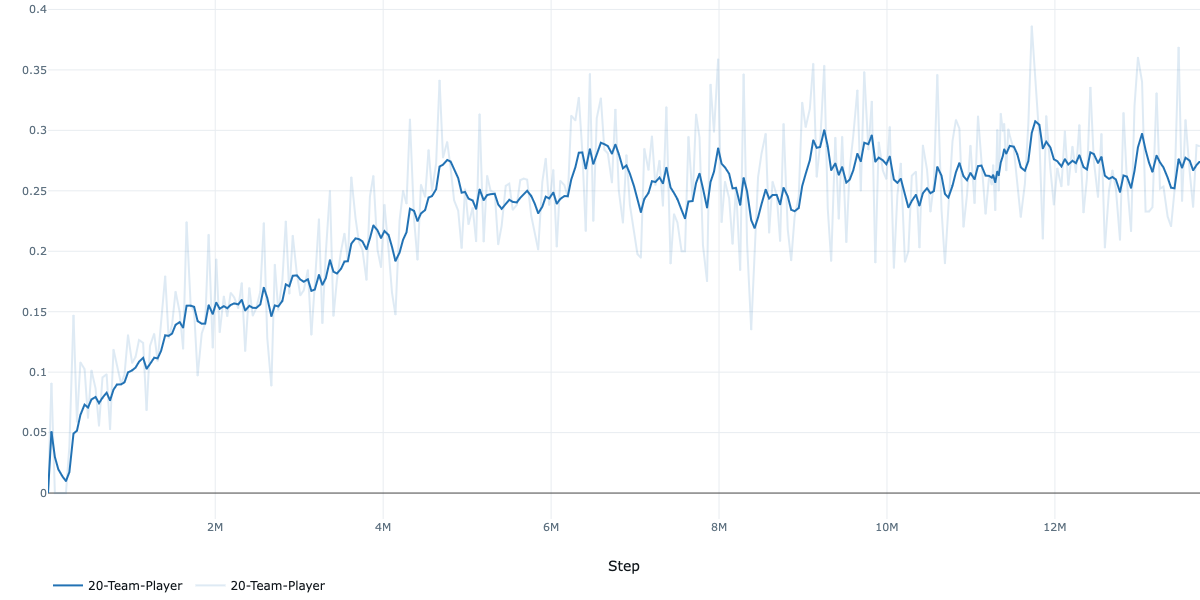
\includegraphics[width=0.95\textwidth]{diagnostics_plots/pool20_outcome_wr_vs_heuristic.png}
  \caption{Fixed 20-team pool: outcome win rate vs.\ heuristic over training steps (plateau around 30\,\%).}
  \label{fig:pool20_heuristic_wr}
\end{figure}

\begin{figure}[H]
  \centering
  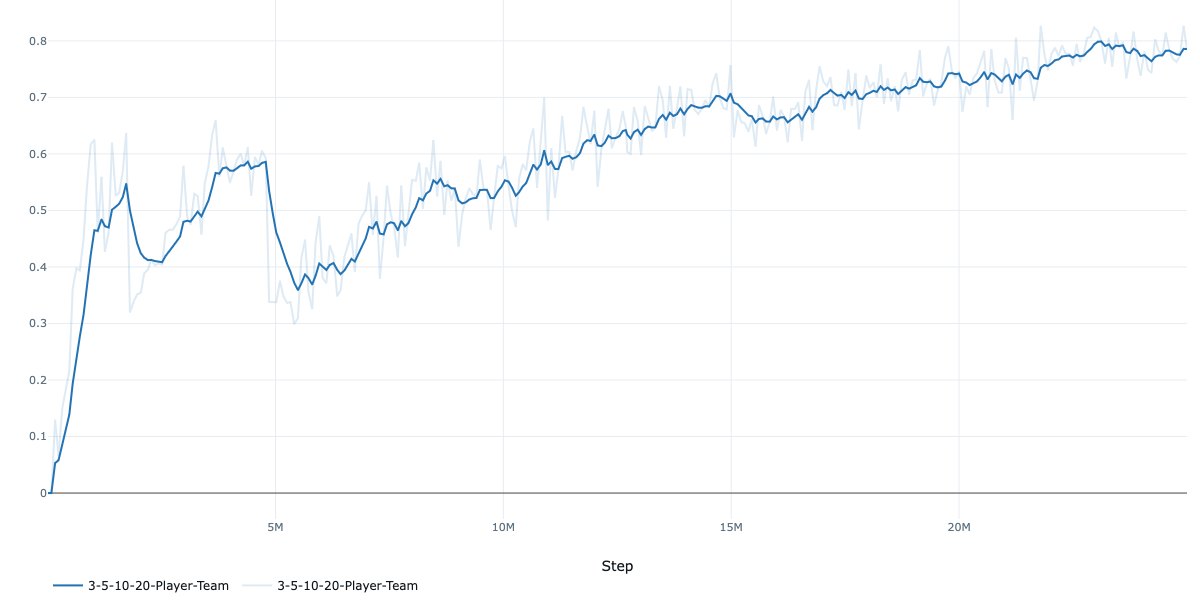
\includegraphics[width=0.95\textwidth]{diagnostics_plots/pool_3_5_10_20_outcome_wr_vs_heuristic.png}
  \caption{Staged pool curriculum ($3 \to 5 \to 10 \to 20$ teams): outcome win rate vs.\ heuristic over training steps (climbing to $\sim$80\,\%).}
  \label{fig:pool_3_5_10_20_heuristic_wr}
\end{figure}

\begin{figure}[H]
  \centering
  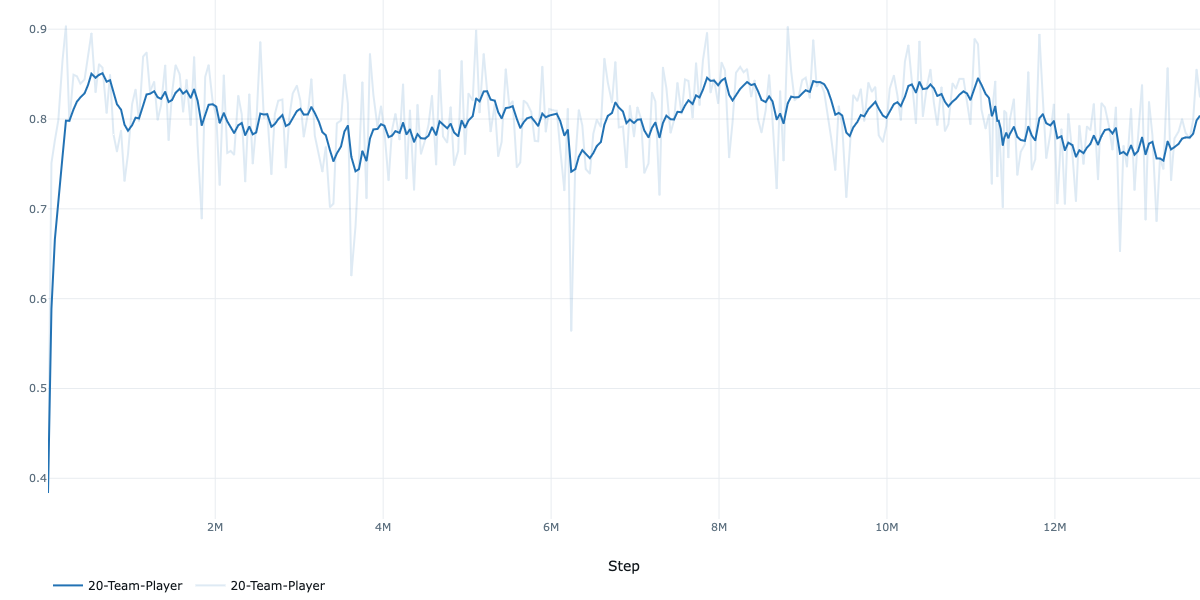
\includegraphics[width=0.95\textwidth]{diagnostics_plots/pool20_explained_variance.png}
  \caption{Fixed 20-team pool: PPO explained variance over training steps (exported from MLflow).}
  \label{fig:pool20_explained_variance}
\end{figure}

\begin{figure}[H]
  \centering
  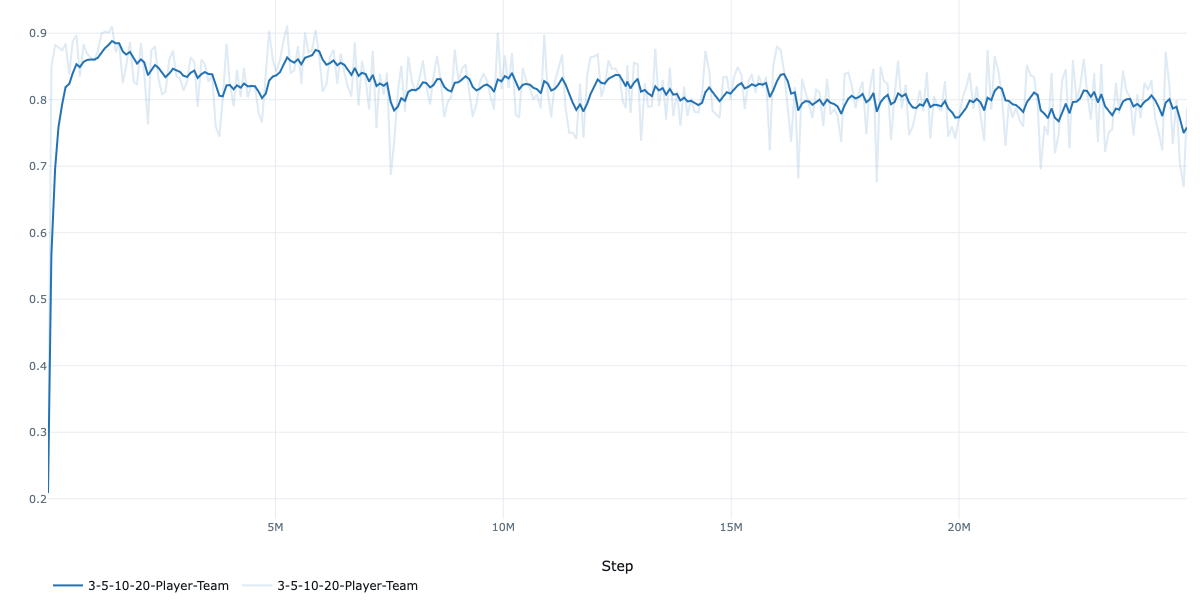
\includegraphics[width=0.95\textwidth]{diagnostics_plots/pool_3_5_10_20_explained_variance.png}
  \caption{Staged pool curriculum ($3 \to 5 \to 10 \to 20$ teams): PPO explained variance over training steps (exported from MLflow).}
  \label{fig:pool_3_5_10_20_explained_variance}
\end{figure}

A checkpoint export for the 25M run is in \texttt{saved\_models/pure\_league\_play\_25M/}.

\begin{figure}[H]
  \centering
  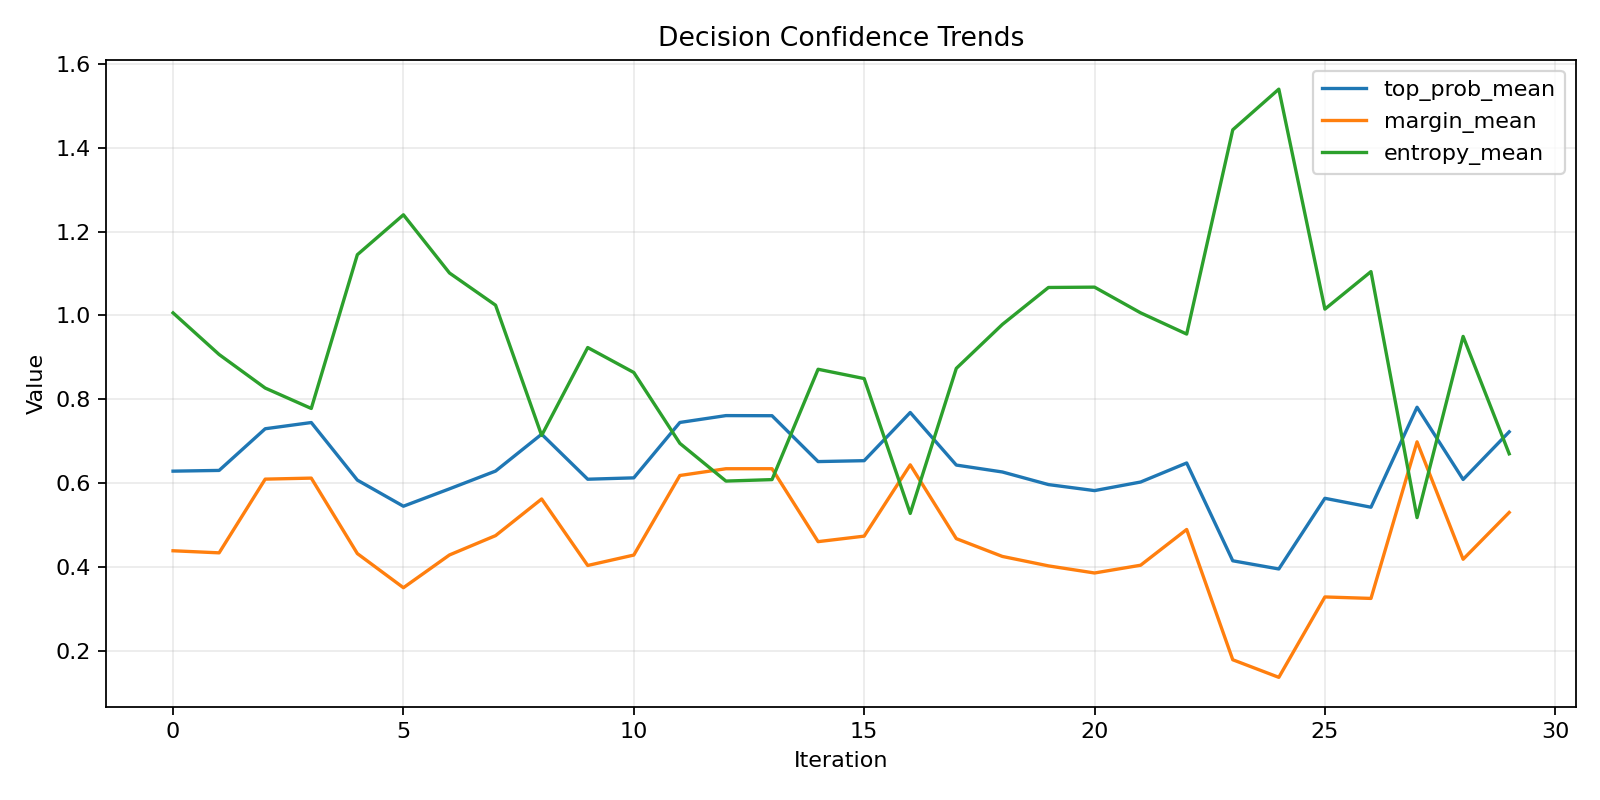
\includegraphics[width=0.95\textwidth]{diagnostics_plots/confidence_trends.png}
  \caption{Decision-diagnostics confidence trends from the final checkpoint (sampled battles; not a training-time metric).}
\end{figure}

\begin{figure}[H]
  \centering
  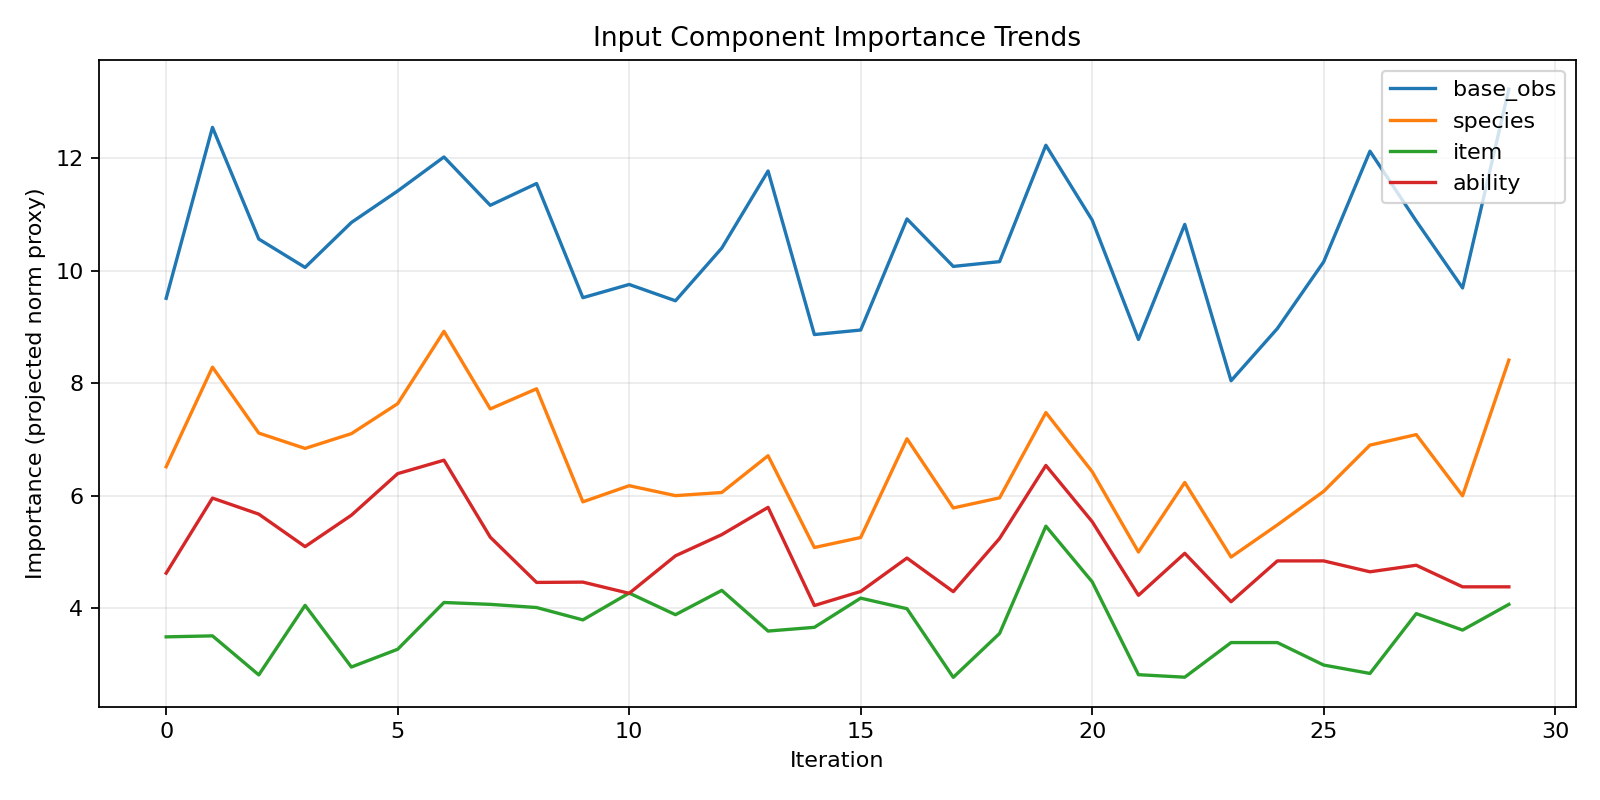
\includegraphics[width=0.95\textwidth]{diagnostics_plots/component_importance_trends.png}
  \caption{Decision-diagnostics input component importance trends from the final checkpoint.}
\end{figure}

\begin{figure}[H]
  \centering
  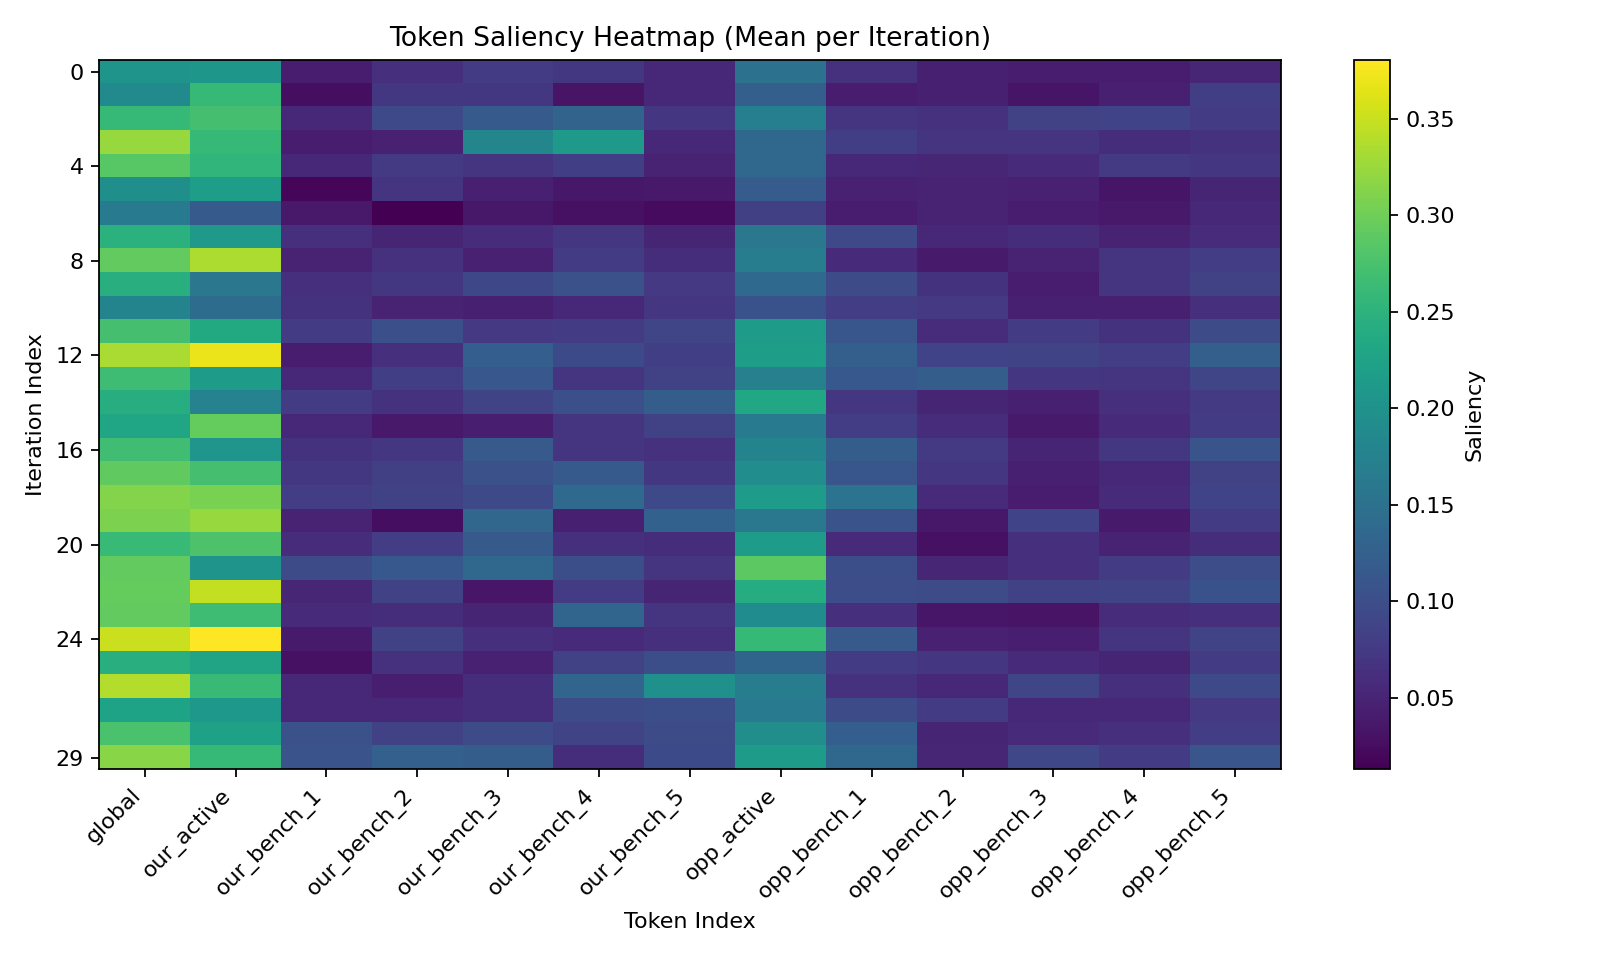
\includegraphics[width=0.85\textwidth]{diagnostics_plots/token_saliency_heatmap.png}
  \caption{Decision-diagnostics token saliency heatmap (final checkpoint).}
\end{figure}

\section{Random Teams (Milestone~2)}

With randomly generated teams for both sides (the standard
\texttt{gen8randombattle} format), the problem is substantially harder.  Each
battle involves unseen teams on both sides (the agent can see its own team),
requiring the agent to generalise rather than memorise a single team's
strategy.

\subsection{Current Best Results}

\begin{center}
\small
\begin{tabularx}{0.8\textwidth}{l c}
  \toprule
  \textbf{Metric} & \textbf{Value} \\
  \midrule
  Benchmark skill score (best trial) & 0.3733 \\
  Win rate vs.\ random              & 84\% \\
  Win rate vs.\ \texttt{random\_no\_switch} & 48\% \\
  Win rate vs.\ heuristic           & 8\,\% \\
  \bottomrule
\end{tabularx}
\end{center}

% TODO: Fill in the per-opponent win rates for the best random-teams trial
% once the hp sweep completes.  Replace the --- entries above.

The skill score of 0.3733 reflects the difficulty of generalisation: the
agent can beat random opponents reliably but struggles against the heuristic.
This is expected given the high entropy in team composition.  However the performance against random\_no\_switch is still very disappointing.

\subsection{Hyperparameter Sweep Status}

The Optuna sweep was made with the following setup:
\begin{itemize}
  \item 50~trials planned, 600K steps per trial.
  \item Single fixed curriculum stage (no promotion), ensuring comparable
        evaluation across trials.
  \item Objective: benchmark skill score.
\end{itemize}

Results were lackluster as there were no major brekthrough findings or large divergences in capability with random teams.

% TODO: Insert Optuna visualisation once sweep completes:
% - Parallel coordinate plot or importance plot showing which hyperparameters
%   most affect the skill score.
% - Best trial's training curves compared to default config.

\subsection{Noise in Benchmark Scores}

An important observation is that the benchmark skill score has significant
variance due to the stochastic nature of random-team battles.  Lucky team
matchups can inflate the score above what the peak training win rates would
imply.  With only 50~episodes per opponent tier, the Wilson confidence
intervals are wide, particularly for the heuristic tier where win rates are
low.  Future work should increase episode counts for more stable evaluation.

\section{Key Insight: Reward Scaling as the Catalyst}

The central finding from the experimental programme is that \textbf{reward
scaling was the single most impactful change}:

\begin{keyinsight}
For the entire project history, the value function was non-functional
(explained variance ${\sim}0.1$) despite multiple architectural improvements.
A single change, adding \texttt{reward\_scale}$\,=0.1$ to normalise returns
from $[-15,+15]$ to $[-1.5,+1.5]$, caused explained variance to jump to
0.53--0.87 and unlocked competency against heuristic opponents (fixed teams).  Combined with
fixed teams, this produced a benchmark skill score of 0.9911 with 98\,\% win
rate vs.\ heuristic.

The lesson: \textbf{normalise the return scale before tuning anything else.}
The value function must be able to learn before the policy can improve.
\end{keyinsight}

This redirects the optimisation focus for the random-teams setting from
architecture to training dynamics: the same reward-scaling insight applies,
but the higher entropy of random teams requires additional work on
generalisation. This problem remains unsolved for now.

\section{Honest Assessment}

At the time of writing, the project demonstrates:

\begin{center}
\small
\begin{tabularx}{\textwidth}{l X}
  \toprule
  \textbf{What works} & \textbf{What still needs work} \\
  \midrule
  Fixed teams: near-perfect performance (skill score 0.99) &
    Random teams: 0.37 skill score, 8\,\% vs.\ heuristic \\
  Value function learns after reward scaling (EV 0.72) &
    Benchmark score has high variance at 50 eps/tier \\
  Self-play infrastructure functional (0\,\% fallback) &
    LSTM end-to-end validation showed no improvement in performance \\
  Distributed training stable at 48 environments &
    Gauntlet validation pipeline not yet automated \\
  MLflow tracking produces complete, comparable metrics &
    Complete information random vs random as a test \\
  Curriculum learning provides structured progression &
    Team builder (Milestone~3) not yet started \\
  \bottomrule
\end{tabularx}
\end{center}

The engineering foundation is solid and Milestone~1 (fixed teams) is
essentially solved.  The remaining work focuses on Milestone~2 (random teams)
and the team builder for Milestone~3 is out of scope.
